%% ****** Start of file apstemplate.tex ****** %
%%
%%
%%   This file is part of the APS files in the REVTeX 4.2 distribution.
%%   Version 4.2a of REVTeX, January, 2015
%%
%%
%%   Copyright (c) 2015 The American Physical Society.
%%
%%   See the REVTeX 4 README file for restrictions and more information.
%%
%
% This is a template for producing manuscripts for use with REVTEX 4.2
% Copy this file to another name and then work on that file.
% That way, you always have this original template file to use.
%
% Group addresses by affiliation; use superscriptaddress for long
% author lists, or if there are many overlapping affiliations.
% For Phys. Rev. appearance, change preprint to twocolumn.
% Choose pra, prb, prc, prd, pre, prl, prstab, prstper, or rmp for journal
%  Add 'draft' option to mark overfull boxes with black boxes
%  Add 'showkeys' option to make keywords appear
\documentclass[aps,prl,twocolumn,groupedaddress]{revtex4-2}
%\documentclass[aps,prl,preprint,superscriptaddress]{revtex4-2}
%\documentclass[aps,prl,reprint,groupedaddress]{revtex4-2}
\usepackage{natbib}
\usepackage[export]{adjustbox}
\usepackage{graphicx}
\usepackage{float}
\usepackage{braket}
\usepackage[utf8]{inputenc}
\usepackage{ctex}
\usepackage{amsmath}
\usepackage{amsbsy}
\usepackage{amsfonts}

% You should use BibTeX and apsrev.bst for references
% Choosing a journal automatically selects the correct APS
% BibTeX style file (bst file), so only uncomment the line
% below if necessary.
%\bibliographystyle{apsrev4-2}

\begin{document}

% Use the \preprint command to place your local institutional report
% number in the upper righthand corner of the title page in preprint mode.
% Multiple \preprint commands are allowed.
% Use the 'preprintnumbers' class option to override journal defaults
% to display numbers if necessary
%\preprint{}

%Title of paper
\title{HHL算法及其应用}

% repeat the \author .. \affiliation  etc. as needed
% \email, \thanks, \homepage, \altaffiliation all apply to the current
% author. Explanatory text should go in the []'s, actual e-mail
% address or url should go in the {}'s for \email and \homepage.
% Please use the appropriate macro foreach each type of information

% \affiliation command applies to all authors since the last
% \affiliation command. The \affiliation command should follow the
% other information
% \affiliation can be followed by \email, \homepage, \thanks as well.
\author{林照翔}
%\email[]{Your e-mail address}
%\homepage[]{Your web page}
%\thanks{}
%\altaffiliation{}
\affiliation{2022级理论物理2班 320220935801}

%Collaboration name if desired (requires use of superscriptaddress
%option in \documentclass). \noaffiliation is required (may also be
%used with the \author command).
%\collaboration can be followed by \email, \homepage, \thanks as well.
%\collaboration{}
%\noaffiliation

\begin{abstract}
% insert abstract here
本文从基本物理概念出发,介绍了 HHL 算法的基本原理,并通过一个数值实例的计算加深了读者对 HHL 算法求解线性系统问题的理解。比较了 HHL 算法与经典最优算法--共轭梯度法在求解线性系统问题时的计算复杂度,发现 HHL 算法相较于共轭梯度法有指数级加速,因此能够大大提高求解线性系统问题的速度。此外,介绍了超导量子计算、拓扑量子计算、光量子计算、囚禁离子量子计算和硅基量子计算的技术前景和实现难点,并简要介绍了 HHL 算法的两个实际应用:量子主成分分析和量子支持向量机。在这个大数据时代,HHL 算法大有可为。
\end{abstract}

% insert suggested keywords - APS authors don't need to do this
%\keywords{}

%\maketitle must follow title, authors, abstract, and keywords
\maketitle

% body of paper here - Use proper section commands
% References should be done using the \cite, \ref, and \label commands
\section{1. 引言}

HHL算法是由 Harrow, Hassidim 和 Lloyd 提出的一种求解量子线性系统的量子算法,其利用量子态的相干叠加与纠缠等特性实现稀疏线性方程组 $A\vec{x}=\vec{b}$ 的快速求解,与经典的线性方程组求解算法相比在特定情况下可以达到指数级加速。求解线性方程组是解决很多量子应用相关问题的基础,因此 HHL 算法是许多复杂量子算法的基本组成部分,且广泛应用于量子支持向量机、量子判别分析、量子线性回归、量子无监督学习、量子神经网络等量子机器学习算法中。在大数据时代,HHL 算法带来的加速收益相当可观。

本文第2节简要介绍了一些量子计算的基本物理概念;第3节详细介绍了 HHL 算法的基本原理;并在第4节通过一个数值实例加深读者对 HHL 算法的理解;第5节比较了 HHL 算法与经典最优算法--共轭梯度法的计算复杂度,发现 HHL 算法相较于共轭梯度法有指数级加速;第6节介绍了量子计算实现平台;第7节简要介绍了 HHL 算法的两个应用:量子主成分分析和量子支持向量机;第8节对全文作了总结;第9节是本文的参考文献。

% Put \label in argument of \section for cross-referencing
%\section{\label{}}

\section{2. 基本物理概念}

本节将对本文涉及的基本物理概念进行简要阐述。

\subsection{A. bra-ket 记号}

量子力学中,用 ket $\ket{\psi}$ 表示一个纯态,用 bra $\bra{\psi}$ 表示其厄米共轭 $\bra{\psi}=(\ket{\psi})^\dag$。若 $\ket{\psi}$ 的矩阵表示为 $\ket{\psi}=\begin{pmatrix} 1\\ -\mathrm{i} \end{pmatrix}$,则 $\bra{\psi}=\begin{pmatrix} 1 &-\mathrm{i} \end{pmatrix}$。

\subsection{B. Hadamard 门}

Hadamard 门常用于构造等概率叠加态,其矩阵表示为

$$
H=\frac{1 }{\sqrt{2} } \begin{pmatrix}
1 &1 \\
1 &-1
\end{pmatrix}
$$

Hadamard 门分别作用于 $\ket{0},\ket{1}$ 上,得到

$$
H\ket{0}
=\frac{1 }{\sqrt{2} }
\begin{pmatrix}
1 &1 \\
1 &-1
\end{pmatrix}
\begin{pmatrix}
1 \\
0
\end{pmatrix}
=\frac{1 }{\sqrt{2} }
\begin{pmatrix}
1 \\
1
\end{pmatrix}
=\frac{1 }{\sqrt{2} } (\ket{0}+\ket{1})
$$

$$
H\ket{1}
=\frac{1 }{\sqrt{2} }
\begin{pmatrix}
1 &1 \\
1 &-1
\end{pmatrix}
\begin{pmatrix}
0 \\
1
\end{pmatrix}
=\frac{1 }{\sqrt{2} }
\begin{pmatrix}
1 \\
-1
\end{pmatrix}
=\frac{1 }{\sqrt{2} } (\ket{0}-\ket{1})
$$

\subsection{C. 纠缠}

若量子态无法写成几个量子比特的张量积的形式,则称这个量子态是纠缠的。例如

$$
\ket{\Psi}=\frac{1 }{\sqrt{2} } (\ket{00}+\ket{11})
$$

就是一个纠缠态。

\subsection{D. 受控操作}

受控操作至少需要两个量子比特。一部分量子比特作为控制位,另一部分量子比特作为靶位。只有当控制位的量子比特满足一定条件时才对靶位执行特定非恒等操作,否则保持靶位不变。

\subsection{E. 量子傅里叶变换(QFT)}

量子傅里叶变换(QFT)把状态 $\ket{x_{n-1}x_{n-2}\cdots x_0} $ 变换为

$$
\begin{aligned}
&\mathrm{QFT}\ket{x_{n-1}x_{n-2}\cdots x_0}= \\
&\frac{1 }{2^{n/2} } \left(\ket{0} + \mathrm{e}^{2\pi\mathrm{i}\left[0.x_{n-1} \right]}\ket{1} \right) \otimes \\
&\left(\ket{0} + \mathrm{e}^{2\pi\mathrm{i}\left[0.x_{n-2}x_{n-1} \right]}\ket{1} \right) \otimes\cdots \otimes \\
&\left(\ket{0}+\mathrm{e}^{2\pi\mathrm{i}\left[0.x_0,\cdots x_{n-2}x_{n-1}\right]}\ket{1} \right)
\end{aligned}
$$

上面是量子傅里叶变换的二进制表述,其等价于下面的十进制表述

$$
\begin{aligned}
\mathrm{QFT}\ket{x}
=\frac{1 }{2^{n/2} } \sum_{y=0}^{2^n-1} \mathrm{e}^{2\pi\mathrm{i} x y / 2^n}\ket{y}
\end{aligned}
$$

\subsection{F. 逆量子傅里叶变换(IQFT)}

逆量子傅里叶变换(IQFT)的十进制表述为

$$
\mathrm{IQFT}\ket{x}
=\frac{1 }{2^{n/2} } \sum_{y=0}^{2^n-1} \mathrm{e}^{-2\pi\mathrm{i} x y / 2^n}\ket{y}
$$

例如,

$$
\begin{aligned}
\mathrm{IQFT}\ket{10}
&=\mathrm{IQFT}\ket{2}
=\frac{1 }{2^{2/2} } \sum_{y=0}^{2^2-1} \mathrm{e}^{-2\pi\mathrm{i}2y/2^2}\ket{y} \\
&=\frac{1 }{2 } \left(\ket{0}-\ket{1}+\ket{2}-\ket{3} \right) \\
&=\frac{1 }{2 } \left(\ket{00}-\ket{01}+\ket{10}-\ket{11} \right)
\end{aligned}
$$

\section{3. HHL算法基本原理}

\subsection{A. 定义和总览}

一个线性系统问题(linear system problem, LSP)可以表述为

$$
A\vec{x} = \vec{b}
$$

其中 $A $ 是  $N_b\times N_b$ 厄米矩阵,$\vec{x},\vec{b}$ 是 $N_b$ 维矢量,$N_b=2^{n_b}$。$\vec{x}$ 或 $\vec{b}$ 是归一化的。$A$ 和 $\vec{b}$ 是已知的,而 $\vec{x}$ 待求解。

HHL 算法包含五个主要组成部分:初态制备、量子相位估计(quantum phase estimation, QPE)、辅助量子比特旋转、逆量子相位估计(inverse quantum phase estimation, IQPE) 和测量。

\begin{figure*}[htbp]
    \centering
    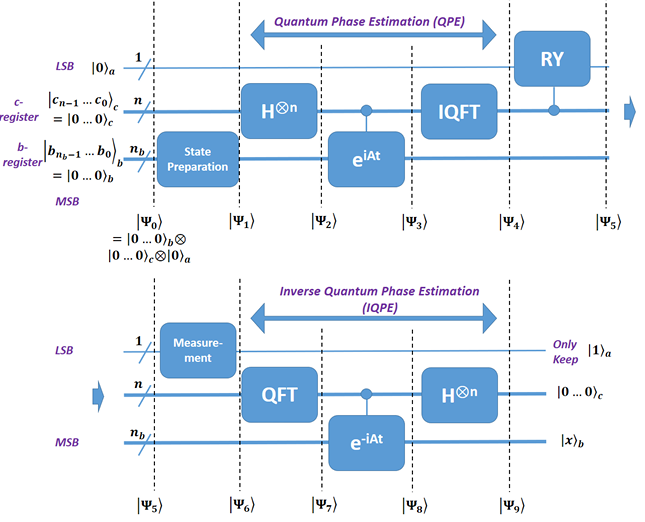
\includegraphics[width=0.70\textwidth]{fig/fig1.png}
    \caption{HHL算法量子线路}
    \label{fig1}
\end{figure*}

HHL 算法中,$\vec{b},\vec{x} $ 的 $N_b$ 个分量编码为 $n_b$ 个量子比特的概率幅。这些量子比特称为 b-寄存器 $\ket{}_b$。

除此之外还有 c-寄存器 $\ket{}_c$,用于储存矩阵 $A$ 在量子相位估计后得到的本征值。

最后一部分是辅助量子比特 $\ket{}_a$。

设厄米矩阵 $A$ 的本征态和本征值分别为 $\left\{\ket{u_i} \right\}$ 和 $\left\{\lambda_i \right\}$,则 $A$ 可进行谱分解

$$
A = \sum_{i=0}^{2^{n_b}-1} \lambda_i \ket{u_i}\bra{u_i}
$$

$A$ 是对角的,因此容易得到 $A^{-1}$

$$
A^{-1} = \sum_{i=0}^{2^{n_b}-1} \lambda_i^{-1} \ket{u_i}\bra{u_i}
$$

$\ket{b}$ 可以表达为

$$
\ket{b} = \sum_{j=0}^{2^{n_b}-1} b_j \ket{u_j}
$$

因此,由方程 $A\ket{x}=\ket{b}$ 有

$$
\ket{x} = A^{-1}\ket{b} = \sum_{i=0}^{2^{n_b}-1} \lambda_i^{-1}b_i \ket{u_i}
$$

由于 $\ket{x}$ 或 $\ket{b}$ 是归一的,因此有归一化条件

$$
\sum_{j=0}^{2^{n_b}-1}\left|b_j \right|^2 = 1
$$

或

$$
\sum_{i=0}^{2^{n_b}-1} \left|\lambda_i^{-1}b_i\right|^2 = 1
$$

\subsection{B. 初态制备}

整个系统共有 $n_b+n+1$ 个量子比特,初始状态为

$$
\ket{\Psi_0}
=\ket{0\cdots 0}_b\ket{0\cdots 0}_c\ket{0}_a
=\ket{0}^{\otimes n_b}\ket{0}^{\otimes n}\ket{0}
$$

设 $\vec{b} = \left(\beta_0,\beta_1,\cdots,\beta_{N_b-1} \right)^{\mathrm{T}} $则 b-寄存器 $\ket{0\cdots 0}_b$ 需要制备为

$$
\ket{b}
=\beta_0\ket{0}+\beta_1\ket{1}+\cdots\beta_{N_b-1}\ket{N_b-1}
$$

总态变为

$$
\ket{\Psi_1}
=\ket{b}_b\ket{0\cdots 0}_c\ket{0}_a
$$

为了方便,在不引起歧义的情况下,下文中 ket 的下标省略。

\subsection{C. 量子相位估计}

首先,对c-量子比特施加 Hadamard 门,得到

$$
\ket{\Psi_2}
=I^{\otimes n_b}\otimes H^{\otimes n}\otimes I\ket{\Psi_1}=
\ket{b}\frac{1 }{2^{n/2} } (\ket{0}+\ket{1})^{\otimes n} \ket{0}
$$

接着,以 c-量子比特为控制比特,依次对 $\ket{b}$ 施加受控 $U^{2^r}$ 门,其中 $r$ 为 c-量子比特的下标,$U=\mathrm{e}^{\mathrm{i}At}$。

假设 $\ket{b}$ 为 $U$ 的本征态,对应本征值为 $\mathrm{e}^{\mathrm{i}2\pi \phi}$,它们本征方程 $U$ 的本征方程

$$
U\ket{b} = \mathrm{e}^{\mathrm{i}2\pi\phi} \ket{b}
$$

当控制比特为 $\ket{0}$,$\ket{b}$ 不受影响;当控制比特为 $\ket{1}$,$U$ 将作用于 $\ket{b}$。结合本征方程可知,总态变为

$$
\begin{aligned}
\ket{\Psi_3}
&=\ket{b}\otimes \bigg[\frac{1 }{2^{n/2} } \left(\ket{0}+\mathrm{e}^{\mathrm{i}2\pi \phi 2^{n-1}}\ket{1} \right)\otimes \\
&\left(\ket{0}+\mathrm{e}^{\mathrm{i}2\pi \phi 2^{n-2}}\ket{1} \right)\otimes \cdots \otimes \left(\ket{0}+\mathrm{e}^{\mathrm{i}2\pi \phi 2^0}\ket{1} \right) \bigg]\otimes\ket{0}_a \\
&=\ket{b} \otimes \left(\frac{1 }{2^{n/2} } \sum_{k=0}^{2^n-1} \mathrm{e}^{2\pi\mathrm{i}\phi k} \ket{k} \right)\otimes \ket{0}_a
\end{aligned}
$$

\begin{figure}[htbp]
    \centering
    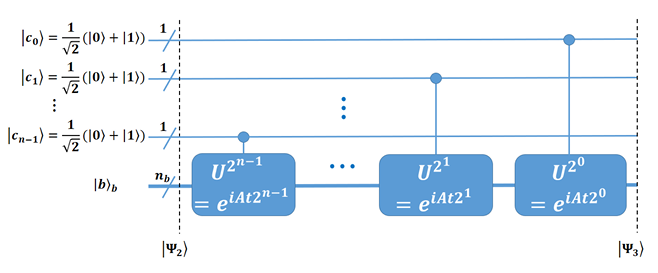
\includegraphics[width=0.55\textwidth]{fig/fig2.png}
    \caption{量子相位估计的受控旋转部分}
    \label{fig2}
\end{figure}

然后对 c-量子比特施加逆量子傅里叶变换(IQFT),总态变为

$$
\begin{aligned}
\ket{\Psi_4}
&=\ket{b}\mathrm{IQFT}\left(\frac{1 }{2^{n/2} } \sum_{k=0}^{2^n-1} \mathrm{e}^{2\pi\mathrm{i}\phi k} \ket{k} \right) \ket{0}_a \\
&=\ket{b}\frac{1 }{2^{n/2} } \sum_{k=0}^{2^n-1} \mathrm{e}^{2\pi\mathrm{i}\phi k} \mathrm{IQFT}(\ket{k}) \ket{0}_a \\
&=\ket{b}\frac{1 }{2^{n/2} } \sum_{k=0}^{2^n-1} \mathrm{e}^{2\pi\mathrm{i}\phi k} \left(\frac{1 }{2^{n/2} } \sum_{y=0}^{2^n-1} \mathrm{e}^{-\mathrm{i}2\pi yk/N} \ket{y} \right) \ket{0}_a \\
&=\frac{1 }{2^n } \ket{b} \sum_{y=0}^{2^n-1}\sum_{k=0}^{2^n-1}\mathrm{e}^{\mathrm{i}2\pi k(\phi-y/N)}\ket{y}\ket{0}_a
\end{aligned}
$$

由上式可见,只有当 $\ket{y}$ 满足条件 $\phi-y/N=0$ 才贡献有限振幅 $\displaystyle{\sum_{k=0}^{2^n-1} \mathrm{e}^0 = 2^n }$,其他情况下贡献的振幅为零,即 $\displaystyle{\sum_{k=0}^{2^n-1}\mathrm{e}^{\mathrm{i}2\pi k (\phi-y/N)}=0,\phi-y/N\ne 0 }$,因此 $\ket{\Psi_4}$ 可以写为

$$
\ket{\psi_4}
=\frac{1 }{2^n } \ket{b} \sum_{k=0}^{2^n-1} \mathrm{e}^{\mathrm{i}2\pi k\cdot 0} \ket{N\phi}\ket{0}_a
=\ket{b}\ket{N\phi}\ket{0}_a
$$

因此,c-量子比特就储存了 $U$ 的本质值 $\mathrm{e}^{\mathrm{i}2\pi \phi} $ 的相位 $\phi$,精确度取决于用于储存的量子比特的数量 $n$。

由于 $U$ 与 $A$ 的关系为 $U = \mathrm{e}^{\mathrm{i}At}$,若 $\ket{b}=\ket{u_j}$ 则

$$
U\ket{b} = \mathrm{e}^{\mathrm{i}\lambda_j t} \ket{b}
$$

与 $U\ket{b}=\mathrm{e}^{\mathrm{i}2\pi \phi}\ket{b}$ 对比,得到 $\phi=\lambda_j t/2\pi$,于是

$$
\ket{\Psi_4}
=\ket{u_j} \ket{N\lambda_j t/2\pi}\ket{0}_a
$$

因此 $A$ 的本征值就编码到了 c-量子比特上。上面的推导均在 $\ket{b}$ 为 $A$ 的某一本征态的假设下进行。一般地,$\ket{b}$ 为 $A$ 的所有本征态的线性叠加,则

$$
\ket{\Psi_4}
=\sum_{j=0}^{2^{n_b}-1} b_j\ket{u_j}\ket{N\lambda_j t/2\pi} \ket{0}_a
$$

通常 $\lambda_j$ 不是整数。选择 $t$ 使得 $\tilde{\lambda}_j\equiv N\lambda_j t/2\pi$ 为整数,则 $\ket{\Psi_4} $ 可写为

$$
\ket{\Psi_4}
=\sum_{j=0}^{2^{n_b}-1} b_j \ket{u_j} \ket{\tilde{\lambda}_j}\ket{0}_a
$$

\subsection{D. 受控旋转和辅助比特的测量}

下一步要基于 c-量子比特储存的本征值来旋转辅助比特 $\ket{0}_a$,总态变为

$$
\ket{\Psi_5}
=\sum_{j=0}^{2^{n_b}-1}b_j\ket{u_j}\ket{\tilde{\lambda}_j}\left(\sqrt{1-\frac{C^2 }{\tilde{\lambda}_j^2 } }\ket{0}_a + \frac{C }{\tilde{\lambda_j} }\ket{1}_a \right)
$$

其中 $C$ 是常数。

当对辅助量子比特进行测量时,其会塌缩至 $\ket{0}$ 或 $\ket{1}$。若其塌缩至 $\ket{0}$,则重复上面过程直至其塌缩为 $\ket{1}$。最终,总态塌缩至

$$
\ket{\Psi_6}
=\frac{1 }{\sqrt{\sum\limits_{j=0}^{2^{n_b}-1}\left|b_j C/\tilde{\lambda}_j \right|^2} }\sum_{j=0}^{2^{n_b}-1}b_j \ket{u_j}\ket{\tilde{\lambda}_j}\frac{C }{\tilde{\lambda}_j }\ket{1}_a
$$

其中,前面多出的系数是归一化因子。

\subsection{E. 非计算(uncomputation)-逆量子相位估计(IQPE)}

非计算通过逆量子相位估计来完成。

首先对 c-量子比特进行量子傅里叶变换,总态变为

$$
\begin{aligned}
\ket{\Psi_7}
&=\frac{1 }{\sqrt{\sum\limits_{j=0}^{2^{n_b}-1}\left|b_j C/\tilde{\lambda}_j \right|^2} }\sum_{j=0}^{2^{n_b}-1}\frac{b_j C }{\tilde{\lambda}_j }  \ket{u_j}\mathrm{QFT}(\ket{\tilde{\lambda}_j})\ket{1}_a \\
&=\frac{1 }{\sqrt{\sum\limits_{j=0}^{2^{n_b}-1}\left|b_j C/\tilde{\lambda}_j \right|^2} }\sum_{j=0}^{2^{n_b}-1}\frac{b_j C }{\tilde{\lambda}_j }  \ket{u_j}\otimes \\
&\left(\frac{1 }{2^{n/2} } \sum_{y=0}^{2^n-1} \mathrm{e}^{\mathrm{i}2\pi y\tilde{\lambda}_j/N} \ket{y} \right) \ket{1}_a\\
\end{aligned}
$$

接着以 c-量子比特为控制比特对 b-寄存器施加逆受控旋转。当第 $r$ 个控制量子比特为 $\ket{0}$ 时,$\ket{u_j}$ 不变;当第 $r$ 个控制量子比特为 $\ket{1}$ 时,对 $\ket{u_j}$ 施加 $\left(U^{-1} \right)^{2^r}$, $U^{-1}=\mathrm{e}^{-\mathrm{i}At}$。于是,总态变为

$$
\begin{aligned}
\ket{\Psi_8}
&=\frac{1 }{2^{n/2}\sqrt{\sum\limits_{j=0}^{2^{n_b}-1}\left|b_j C/\tilde{\lambda}_j \right|^2} } \sum_{j=0}^{2^{n_b}-1}\frac{b_j C }{\tilde{\lambda}_j }\ket{u}_j \sum_{y=0}^{2^n-1}\ket{y}\ket{1}_a \\
&=\frac{C }{2^{n/2}\sqrt{\sum\limits_{j=0}^{2^{n_b}-1}\left|b_j C/\lambda_j \right|^2} } \ket{x} \sum_{y=0}^{2^n-1} \ket{y}\ket{1}_a
\end{aligned}
$$

最后,对 c-量子比特施加 Hadamard 门,得到

$$
\begin{aligned}
\ket{\Psi_9}
&=\frac{1 }{\sqrt{\sum\limits_{j=0}^{2^{n_b}-1}\left|b_j C/\lambda_j \right|^2} }\sum_{j=0}^{2^{n_b}-1} \frac{b_j C }{\lambda_j } \ket{u_j}\ket{0}^{\otimes n}\ket{1}_a \\
&=\frac{C }{\sqrt{\sum\limits_{j=0}^{2^{n_b}-1}\left|b_j C/\lambda_j \right|^2} }\ket{x}_b\ket{0}_c^{\otimes n}\ket{1}_a
\end{aligned}
$$

若 $C$ 为实数,利用归一化条件 $\displaystyle{\sum_{j=0}^{2^{n_b}-1}\left|\lambda_j^{-1}b_j \right|^2=1 }$ 得到

$$
\ket{\Psi_9}
=\ket{x}_b\ket{0}_c^{\otimes n}\ket{1}_a
$$

最终,经一系列操作后,解 $\ket{x}$ 储存在 b-寄存器中。

\section{4. HHL算法的数值实例}

\subsection{A. 编码}

在数值实例中,矩阵 $A$ 和矢量 $\vec{b}$ 分别为

$$
A
=\begin{pmatrix}
1 &-1/3 \\
-1/3 &1  
\end{pmatrix},\quad
\vec{b}
=\begin{pmatrix}
0 \\
1
\end{pmatrix}
$$

$A$ 的本征值和本征向量分别为

$$
\lambda_0 = \frac{2 }{3 } ,
\vec{u}_0
=\begin{pmatrix}
-1/\sqrt{2} \\
-1/\sqrt{2}
\end{pmatrix},
\lambda_1 = \frac{4 }{3 } ,
\vec{u}_1
=\begin{pmatrix}
-1/\sqrt{2} \\
1/\sqrt{2}
\end{pmatrix}
$$

需要 $2$ 个量子比特来把 $\lambda_0$ 编码到 $\ket{01}$ 上,$\lambda_1$ 编码到 $\ket{10}$ 上,且保持比值 $\lambda_1/\lambda_0=2$。$\ket{\tilde{\lambda}_0}=\ket{01},\ket{\tilde{\lambda}_1}=\ket{10};n=2;N=4;t=3\pi/4;\tilde{\lambda}_j=N\lambda_j t/2\pi;\tilde{\lambda}_0=1,\tilde{\lambda}_2=2;$

$\vec{b}$ 是 $2$ 向量,可用 $1$ 个量子比特编码,$n_b=1$。

解 $\vec{x} $ 为

$$
\vec{x}
=\begin{pmatrix}
3/8 \\
9/8
\end{pmatrix}
$$

解的两个分量模方的比值为 $\left|x_0 \right|^2/\left|x_1 \right|^2=1/9$。

\subsection{B. 受控U门的实现}

这里 $n=2$,需要两个操作 $U^{2^1}=U^2,U^{2^0}=U$,分别由 $c_1$ 和 $c_0$ 控制。

从原基矢到 $A$ 本征基矢的变换矩阵为

$$
V
=\begin{pmatrix}
\vec{u}_0 &\vec{u}_1 
\end{pmatrix}
=\begin{pmatrix}
-1/\sqrt{2} &-1/\sqrt{2} \\
-1/\sqrt{2} &1/\sqrt{2}
\end{pmatrix}
$$

以 $\vec{u}_0,\vec{u}_1$ 为基,对角化的 $A_{\mathrm{diag}}$ 为

$$
A_{\mathrm{diag}}
=V^\dag A V
=\begin{pmatrix}
2/3 &0 \\
0 &4/3
\end{pmatrix}
$$

对角化的 $U$ 为

$$
U_{\mathrm{diag}}
=\begin{pmatrix}
\mathrm{e}^{\mathrm{i}\lambda_0 t} &0 \\
0 &\mathrm{e}^{\mathrm{i}\lambda_1 t}
\end{pmatrix}
=\begin{pmatrix}
\mathrm{e}^{\mathrm{i}\pi/2} &0 \\
0 &\mathrm{e}^{\mathrm{i}\pi}
\end{pmatrix}
=\begin{pmatrix}
\mathrm{i} &0 \\
0 &-1
\end{pmatrix}
$$

$$
U_{\mathrm{diag}}^2
=\begin{pmatrix}
-1 &0 \\
0 &1
\end{pmatrix}
$$

还原到原基矢,有

$$
U
=V U_{\mathrm{diag}} V^\dag
=\frac{1 }{2 } \begin{pmatrix}
-1+\mathrm{i} &1+\mathrm{i} \\
1+\mathrm{i} &-1+\mathrm{i}
\end{pmatrix}
$$

$$
U^2
=\begin{pmatrix}
0 &-1 \\
-1 &0
\end{pmatrix}
$$

为了实现 $U$ 和 $U^2$,需要如下的 4-参数门

$$
U
=\begin{pmatrix}
\mathrm{e}^{\mathrm{i}\gamma }\cos(\theta/2) &-\mathrm{e}^{\mathrm{i}(\gamma+\lambda)}\sin(\theta/2) \\
\mathrm{e}^{\mathrm{i}(\gamma+\phi)}\sin(\theta/2) &\mathrm{e}^{\mathrm{i}(\gamma+\phi+\lambda)}\cos(\theta/2)
\end{pmatrix}
$$

取 $\theta=\pi,\phi=\pi,\lambda=0,\gamma=0$ 得到 $U$;取 $\theta=\pi/2,\phi=-\pi/2,\lambda=\pi/2,\gamma=3\pi/4$ 得到 $U^2$。

对于逆量子相位估计,需要实现 $U^{-1}$ 和 $\left(U^{-1} \right)^2$,而 $\left(U^{-1} \right)^2=U^2$

$$
U^{-1}
=\frac{1 }{2 } \begin{pmatrix}
-1-\mathrm{i} &1-\mathrm{i} \\
1-\mathrm{i} &-1-\mathrm{i}
\end{pmatrix}
$$

取 $\theta=\pi/2,\phi=\pi/2,\lambda=-\pi/2,\gamma=-3\pi/4$ 得到 $U^{-1}$。

受控 $U'$ 可写为

$$
\mathrm{C}-U'=I\otimes\ket{0}\bra{0} + U'\otimes \ket{1}\bra{1}
$$

例如,受控 $U^{-1}$ 门 $\mathrm{C}-U^{-1}$ 为

$$
\begin{aligned}
\mathrm{C}-U^{-1}
&=\begin{pmatrix}
1 &0 \\
0 &1
\end{pmatrix}\otimes
\begin{pmatrix}
1 &0 \\
0 &0
\end{pmatrix} + \frac{1 }{2 } 
\begin{pmatrix}
-1-\mathrm{i} &1-\mathrm{i} \\
1-\mathrm{i} &-1-\mathrm{i}
\end{pmatrix}\otimes
\begin{pmatrix}
0 &0 \\
0 &1
\end{pmatrix} \\
&=\frac{1 }{2 } 
\begin{pmatrix}
2 &0 &0 &0 \\
0 &-1-\mathrm{i} &0 &1-\mathrm{i} \\
0 &0 &2 &0 \\
0 &1-\mathrm{i} &0 &-1-\mathrm{i}
\end{pmatrix}
\end{aligned}
$$

\subsection{C. 受控旋转辅助量子比特的实现}

辅助量子比特 $\ket{0}$ 和 $\ket{1}$ 前的系数分别为 $\sqrt{1-C^2/\tilde{\lambda}_j^2}$ 和 $C/\tilde{\lambda}_j$,由于 $C\leq \tilde{\lambda_j}$,而 $\tilde{\lambda}_j$ 的最小值为 $1$,因此不妨取 $C=1$。

从 $\ket{0}_a$ 到 $\sqrt{1-\tilde{\lambda}_j^{-2}}\ket{0}_a+\tilde{\lambda}_j^{-1}\ket{1}_a$ 的变换等价于 $\mathrm{RY}(\theta)$ 旋转,

$$
\mathrm{RY}(\theta)
=\begin{pmatrix}
\cos(\theta/2) &-\sin(\theta/2) \\
\sin(\theta/2) &\cos(\theta/2)
\end{pmatrix}
$$

其中,$\theta=2\arcsin\left(\tilde{\lambda}_k^{-1}\right)$。

$$
\begin{aligned}
\mathrm{RY}(\theta)\ket{0}_a
&=\begin{pmatrix}
\cos(\theta/2) &-\sin(\theta/2) \\
\sin(\theta/2) &\cos(\theta/2)
\end{pmatrix}
\begin{pmatrix}
1 \\
0
\end{pmatrix} \\
&=\cos(\theta/2)\ket{0}_a + \sin(\theta/2)\ket{1}_a
\end{aligned}
$$

定义函数

$$
\theta(c) = \theta(c_1c_0) = 2\arcsin\left(\frac{1 }{c }  \right)
$$

其中 $c$ 是十进制数,$c_1c_0$ 是它的二进制表示。

$$
\theta(1) = \theta(01) = 2\arcsin\left(\frac{1 }{1 }  \right) = \pi
$$

$$
\theta(2) = \theta(10) = 2\arcsin\left(\frac{1 }{2 }  \right) = \frac{\pi }{3 } 
$$

此函数的二进制表示为

$$
\theta(c) = \theta(c_1c_0) = \frac{\pi }{3 }c_1 + \pi c_0 
$$

受控旋转实现如下

$$
\begin{aligned}
&\ket{1}\bra{1}\otimes I \otimes \mathrm{RY}\left(\frac{\pi }{3 }  \right) + \ket{0}\bra{0}\otimes I\otimes I + \\ 
&I\otimes\ket{1}\bra{1}\otimes \mathrm{RY}\left(\pi \right) + I\otimes\ket{0}\bra{0}\otimes I
\end{aligned}
$$

\subsection{D. 量子线路}

详细量子线路图请见图3。

\begin{figure*}[htbp]
    \centering
    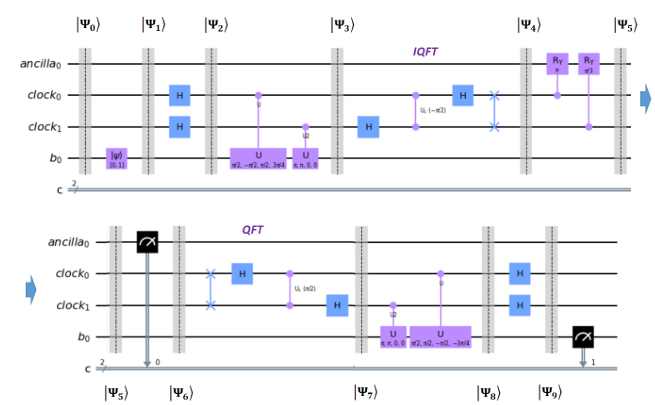
\includegraphics[width=0.75\textwidth]{fig/fig3.png}
    \caption{HHL算法数值实例的量子线路}
    \label{fig3}
\end{figure*}

\subsection{E. 数值替换}

HHL 算法的初态为

$$
\ket{\Psi_0}=\ket{0}_b\otimes\ket{00}_c\otimes\ket{0}_a=\ket{0000}
$$

利用 X-门把 $\ket{0}_b$ 变换为 $\ket{1}_b$

$$
\ket{\Psi_1} = X\otimes I\otimes I\ket{\Psi_0} = \ket{1000}
$$

之后利用 Hadamard 门来构造 c-量子比特的叠加态

$$
\begin{aligned}
\ket{\Psi_2}
&=I\otimes H^{\otimes n}\otimes I \ket{\Psi_1} \\
&=\ket{1}\frac{1 }{2^{2/2} } \left(\ket{0}+\ket{1} \right)^{\otimes 2}\ket{0} \\
&=\frac{1 }{2 } \left(\ket{1000}+\ket{1010}+\ket{1100}+\ket{1110} \right)
\end{aligned}
$$

利用 $\ket{1}=\frac{1 }{\sqrt{2} } \left(-\ket{u_0}+\ket{u}_1 \right)$,$\ket{\Psi_2}$ 可写为

$$
\begin{aligned}
\ket{\Psi_2}
&=\ket{1}\frac{1 }{2 } \left(\ket{000}+\ket{010}+\ket{100}+\ket{110} \right) \\
&=\frac{1 }{2\sqrt{2} } \big(-\ket{u_0}\ket{000}-\ket{u_0}\ket{010}-\ket{u_0}\ket{100} \\
&-\ket{u_0}\ket{110}+\ket{u_1}\ket{000}+\ket{u_1}\ket{010} \\
&+\ket{u_1}\ket{100}+\ket{u_1}\ket{110}\big)
\end{aligned}
$$

在受控旋转操作中,当 c-寄存器为 $\ket{k}_c$ 时,$\ket{u}_j$ 的相位要加上 $\phi_j=k\lambda_j t/2\pi$。这里 $t=3\pi/4,\lambda_0=2/3,\lambda_1=4/3$,因此可得

$$
\begin{aligned}
\ket{\Psi_3}
&=\frac{1 }{2\sqrt{2} } \big[\left(-\ket{u_0}+\ket{u_1} \right)\ket{00} + \left(-\mathrm{i}\ket{u_0}-\ket{u_1} \right)\ket{01} \\
&+\left(\ket{u_0}+\ket{u_1} \right)\ket{10}+\left(\mathrm{i}\ket{u_0}-\ket{u_1} \right)\ket{11} \big]\ket{0}
\end{aligned}
$$

再对 c-量子比特施加逆量子傅里叶变换

$$
\begin{aligned}
\ket{\Psi_4}
&=\mathrm{IQFT}\ket{\Psi_3} \\
&=\frac{1 }{4\sqrt{2} } \big[\left(-\ket{u_0}+\ket{u_1} \right)\left(\ket{00}+\ket{01}+\ket{10}+\ket{11} \right)+\\
&\left(-\mathrm{i}\ket{u_0}-\ket{u_1} \right)\left(\ket{00}-\mathrm{i}\ket{01}-\ket{10}+\mathrm{i}\ket{11} \right)+\\
&\left(\ket{u_0}+\ket{u_1} \right)\left(\ket{00}-\ket{01}+\ket{10}-\ket{11} \right)+\\
&\left(\mathrm{i}\ket{u_0}-\ket{u_1} \right)\left(\ket{00}+\mathrm{i}\ket{01}-\ket{10}-\mathrm{i}\ket{11} \right) \big]\ket{0} \\
&=\frac{1 }{\sqrt{2} } \left(-\ket{u_0}\ket{01}+\ket{u_1}\ket{10} \right)\ket{0}
\end{aligned}
$$

接着旋转辅助量子比特,得到

$$
\begin{aligned}
\ket{\Psi_5}
&=\sum_{j=0}^{2^1-1} b_j\ket{u_j}\Ket{\tilde{\lambda}_j}\left(\sqrt{1-C^2/\tilde{\lambda}_j^2}\ket{0} + \frac{C }{\tilde{\lambda}_j } \ket{1} \right) \\
&=-\frac{1 }{\sqrt{2} } \ket{u_0}\ket{01}\ket{1} + \frac{1 }{\sqrt{2} } \ket{u_1}\ket{10}\left(\frac{\sqrt{3} }{2 } \ket{0} + \frac{1 }{2 } \ket{1} \right) 
\end{aligned} 
$$

对辅助量子比特进行测量,若测得 $\ket{1}$,状态塌缩至

$$
\ket{\Psi_6}
=\sqrt{\frac{8 }{5 } }\left(-\frac{1 }{\sqrt{2} } \ket{u_0}\ket{01}\ket{1} + \frac{1 }{2\sqrt{2} } \ket{u_1}\ket{10}\ket{1} \right)
$$

对 $\ket{\Psi_6}$ 进行量子傅里叶变换,得到

$$
\begin{aligned}
\ket{\Psi_7}
&=\sqrt{\frac{8 }{5 } }\bigg[-\frac{1 }{\sqrt{2} } \ket{u_0}\frac{1 }{2 } \left(\ket{00}+\mathrm{i}\ket{01}-\ket{10}-\mathrm{i}\ket{11} \right)\ket{1} + \\
&\frac{1 }{2\sqrt{2} } \ket{u_1}\frac{1 }{2 } \left(\ket{00}-\ket{01}+\ket{10}-\ket{11} \right) \bigg]\ket{1}
\end{aligned}
$$

对于受控旋转,若 $c_0=1,c_1=1$,则状态要多乘两个相位因子 $\mathrm{e}^{-\mathrm{i}\lambda_j t},\mathrm{e}^{-\mathrm{i}2\lambda_j t}$。这里 $\mathrm{e}^{-\mathrm{i}\lambda_0 t}=-\mathrm{i},\mathrm{e}^{-\mathrm{i}2\lambda_0 t}=-1,\mathrm{e}^{-\mathrm{i}\lambda_1 t}=-1,\mathrm{e}^{-\mathrm{i}2\lambda_1 t}=1;Nt/2\pi=3/2$,于是得到

$$
\begin{aligned}
\ket{\Psi_8}
&=\frac{1 }{2 } \sqrt{\frac{8 }{5 } }\left(-\frac{1 }{\sqrt{2} } \ket{u_0} + \frac{1 }{2\sqrt{2} } \ket{u_1} \right)\otimes \\
&\left(\ket{00}+\ket{01}+\ket{10}+\ket{11} \right)\ket{1}
\end{aligned}
$$

最后再施加 Hadamard 门,得到

$$
\begin{aligned}
\ket{\Psi_9}
&=\frac{2 }{3 } \sqrt{\frac{8 }{5 } }\left(-\frac{1 }{\frac{2 }{3 } \sqrt{2} } \ket{u_0} + \frac{1 }{\frac{4 }{3 } \sqrt{2} } \ket{u_1} \right)\ket{00}\ket{1}
\end{aligned}
$$

利用 $\ket{u_0}=-\frac{1 }{\sqrt{2} }\ket{0}-\frac{1 }{\sqrt{2} } \ket{1},\ket{u_1}=-\frac{1 }{\sqrt{2} } \ket{0} + \frac{1 }{\sqrt{2} \ket{1} } $,$\ket{\Psi_9}$ 化为

$$
\ket{\Psi_9}
=\frac{1 }{2 } \sqrt{\frac{2 }{5 } }\left(\ket{0}_b+3\ket{1}_b \right)\ket{00}_c\ket{1}_a
$$

b-寄存器中 $\ket{0},\ket{1}$ 的概率比为 $1:9$,这与预期相符。

\subsection{5. HHL算法的计算复杂度与经典算法的比较}

求解线性方程组的最优经典算法是共轭梯度法(conjugate-gradiant method),其计算复杂度为 $\mathcal{O}(Ns\kappa \log(1/\varepsilon))$,其中 $s$ 是矩阵的稀疏度,$\kappa$ 是条件数(矩阵最大本征值与最小本征值之比),$\varepsilon$ 是算法精度。

而 HHL 算法的计算复杂度为 $\mathcal{O}(\log(N)s^2\kappa^2/\varepsilon)$,其相较于经典算法实现了对 $N$ 的指数级加速。

\section{6. 量子计算实现平台}

本节介绍超导量子计算、拓扑量子计算、光量子计算、囚禁离子量子计算和硅基量子计算的技术前景和实现难点。

\subsection{A. 超导量子计算}

超导量子比特是由约瑟夫森结和其他超导元器件构成的非线性量子谐振电路,分为以电荷、相位、磁通等自由度编码量子信息的基本类型以及为数众多的复合类型。当前的主流类型之一是 Transmon 及其变种,对环境电荷的涨落敏感,具有较长的退相干时间;其他常见类型有磁通量子比特、Fluxonium、$0-\pi$ 比特等。

超导量子计算路线的优势在于:超导量子芯片的制备工艺与微纳加工技术兼容,具有较好的可扩展性;超导量子比特及相关器件的参数具有良好的设计自由度;超导量子线路的操控使用成熟的微波电子学技术,速度快、可操控性好。

超导量子计算路线面临的挑战主要有三方面。① 主流的平面结构限制了比特之间的连接性,由于只能实现近邻耦合而导致运行量子算法时的极大额外开销,需要改进连接性来精简量子线路的深度。② 超导量子芯片的控制线的数量随着比特数线性增加,但其平面属性导致只能从芯片四周将控制线引入到芯片中央,这在扩展时使得控制线密度不断增大,而串扰将更难抑制。多层芯片三维集成技术可以一定程度上缓解该问题,但在更高集成度情形下解决布线和串扰问题极具挑战性。③ 超导量子比特的退相干时间需要进一步提升,涉从微观机理出发,对材料、设计、工艺、测试环境进行全方位优化。

\subsection{B. 拓扑量子计算}

发展量子计算技术面临的最大挑战是如何解决退相干带来的误差。与其他技术路线相比,拓扑量子计算被认为可在原理层面上解决这一问题。理论上只需少数几个(甚至1个)拓扑量子比特即可构建1个逻辑比特;一旦实现拓扑量子比特,即可进入集成逻辑比特的时代,这将是量子计算发展的飞跃式进步。

目前,用于探索拓扑量子计算的体系包括强自旋轨道耦合材料和s波超导体近邻体系、拓扑绝缘体和s波超导体近邻体系、铁基超导体、本征拓扑超导体。本方向的关键技术有量子材料生长、拓扑量子器件制备、拓扑态的量子输运测量等,相关研究是实现应用突破的关键。

零偏压电导峰曾经被作为判断是否存在马约拉纳量子态的依据,但当前共识是这一依据并不可靠;如何实现满足非阿贝尔统计的编织操作也是本方向亟待解决的核心问题。整体来看,拓扑量子计算尚处基础研究阶段。

\subsection{C. 光量子计算}

光量子系统具有抗退相干、单比特操纵简单精确、提供分布式接口等优点,可以利用光子的多个自由度进行编码,是重要的量子信息处理系统之一。光量子计算可分为专用和通用的量子计算模型;根据编码方式的不同也可分为离散变量和连续变量模型(或二者的结合)。这些不同的路径都有望实现通用量子计算。

光量子计算的核心硬件包括量子光源、光量子线路、单光子探测器。量子光源用于制备特定初始态,常见类型有确定性的单光子源、压缩真空态光源、纠缠光子对光源等。半导体量子点在激光的激发下会像原子一样辐射单个光子,是实现确定性的可扩展单光子源的重要途径。中国科学技术大学研究团队2013年首创量子点脉冲共振激发技术,研制出了确定性偏振、高纯度、高效率的单光子源;2018年实现了高全同性、高受激效率的参量下转换纠缠光子对;2019年实现了高保真度、高效率、高全同性的双光子纠缠源。2020年,研究者首次实现了片上高纯度、高全同性、预报效率大于 90\% 的光源。

早期的光量子计算主要基于自由空间的线性光学,实验技术成熟,光子在晶体和自由空间中的损耗都很低,但此方案的可扩展性较差。大规模扩展的可行路径是将光学元件集成到光芯片上,如将量子光源、线路、探测器全部集成在一个波导芯片。这类光芯片方案稳定性和可扩展性良好,但目前的效率还需提升。相关研究整体上处于起步阶段。

光量子计算路线当前最大的挑战是如何实现确定性的两比特纠缠门,大规模的纠缠态制备和线路操纵、高效率探测器的研制等也是亟待研究的难题。两比特纠缠门的实现思路有两种:基于线性光学,在线性光学的基础上引入非线性。在大规模、可扩展的纠缠态制备方面,有望以量子点自旋为媒介,将辐射单光子制备到大规模纠缠态上。在近期,光量子计算的发展趋势表现为:实现含噪声、中等规模的量子计算应用;实现确定性两比特纠缠门,解决通用光量子计算的瓶颈问题;制备大规模纠缠态;实现基于GKP态的容错量子计算。

\subsection{D. 囚禁离子量子计算}

囚禁离子系统是最早用于量子计算的物理系统,以囚禁在射频电场中离子的超精细或塞曼能级作为量子比特载体,通过激光或微波进行相干操控。离子量子比特的频率只由离子种类、外界磁场决定,因而相比超导、量子点等人造量子比特具有完美的全同性。囚禁在一个势阱中的多个离子在库伦斥力作用下会形成稳定的晶格结构,整个晶格的简谐振动可作为阱中不同离子之间产生量子纠缠的媒介。囚禁离子系统具有全连接性,即系统中任意量子比特间都存在直接相互作用;处于不同阱中的离子还能以各自辐射的光子作为媒介来实现
远程纠缠。

囚禁离子系统的早期发展得益于成熟的原子/分子光学实验技术,并无明显的技术瓶颈。当规模较小时,囚禁离子系统具有小时级的相干时间、极高的量子门保真度。然而,囚禁离子系统在规模化、系统稳定性方面尚存困难,如随着同一势阱中离子数目的增多,离子晶格会愈发不稳定,离子晶格的振动频谱也趋于密集而难以利用。目前,解决这一问题的主流方案是“量子电荷耦合器件(QCCD)架构”,即利用电极在芯片上定义多个囚禁区域,每个区域包含少量离子;通过调制各电极的电压,驱动离子在不同区域之间移动和交换。

QCCD架构的未来发展方向是,在片上集成控制电路、光波导、光探测器,实现系统的集成化和小型化;由于涉及芯片制备、芯片封装、光波导制备、表面处理等多项技术集成,发展难度较大。目前,构建包含数十至上百个离子的中小规模系统没有原理性障碍,但需要解决以下技术性问题:① 光波导、电路、探测器等多器件集成型芯片阱的设计与制备;② 因离子的反常加热率较高限制了门操作的保真度,需要发展低温阱、芯片表面处理等技术来降低加热率;③ 系统的真空、光学、信号控制等部分的耦合度较高,不利于保持整体稳定性,需将各子系统进行模块化和小型化处理。

\subsection{E. 硅基量子计算}

硅基量子计算使用量子点中囚禁的单电子或空穴作为量子比特,通过电脉冲实现对比特的驱动和耦合。这一技术路线的优势表现在:大部分工艺与传统的金属 - 氧化物 - 半导体(MOS)工艺兼容,具有大规模扩展的潜力,在商业化阶段将易于和半导体行业对接;比特相干时间长,门操作精度高;可进行全电学操控。硅基量子点的实现方式分为两种。① 通过在门电极上加载电压来囚禁单个电子或空穴,利用电极对其量子态进行操控;这种方式可实现比特间耦合的可灵活调节,但集成的门电极密度高,需要采用公共和悬浮电极等才能大规模生产。② 通过扫描隧道显微镜(STM)或离子束注入方式在硅衬底中掺杂原子并作为比特载体,然后利用MOS电极或STM直写电极对掺杂原子的电子自旋进行操控;具有比特全同性高、易于扩展、电极密度低、相干时间长等优点,但加工难度大。

近年来,硅基量子计算研究进展迅速,多个研究团队独立实现了3~6个比特的集成;将量子门保真度提升到了容错阈值之上,实现了电子自旋与超导微波腔的强耦合、基于微波光子的长程自旋耦合。最近发展的低温集成 - 互补金属氧化物半导体(Cryo-CMOS)量子测控技术,在与硅基比特结合后有望解决中大规模的读取及控制问题;通过融合硅基量子芯片和经典CMOS低温芯片,多个研究团队实现了在1.1~4 K温区运行良好的硅基热比特。因此,硅基平台是目前唯一可在4 K温度条件下利用大规模集成半导体工艺实现经典 - 量子混合的体系。

硅基量子计算的发展挑战有:单比特门所需元件占据较大空间,应优化比特驱动方案;多量子比特的集成需在方案和技术层面需取得突破;在单原子量子计算方面进一步提升原子放置的精度和成功率以实现单原子阵列;在工艺水平进一步提升后,改善硅基衬底质量和介电层电噪声以提高芯片成品率。

\section{7. HHL算法的应用}

本节简要介绍 HHL 算法在量子主成分分析(quantum principal component analysis, qPCA)和量子支持向量机(quantum support vector machine, qSVM)中的应用。

\subsection{A. 量子主成分分析}

问题:给定一个未知量子态 $\rho$ 的 $n$ 份拷贝,求它的本征值分解。(记 $\rho$ 的本征系为 $\left\{r_i,\ket{\chi_i} \right\}$,$\displaystyle{\rho=\sum_{i} r_i\ket{\chi_i}\bra{\chi_i} }$ )

设有两个寄存器,第一个储存 $\rho$,第二个储存任意密度矩阵 $\sigma$,注意到

$$
\begin{aligned}
&\mathrm{Tr}_1\left(\mathrm{e}^{-\mathrm{i}S\Delta t}\rho\otimes \sigma \mathrm{e}^{\mathrm{i}S\Delta t}\right) \\
=&\left(\cos^2\Delta t \right)\sigma + \left(\sin^2\Delta t \right)\rho - \mathrm{i}\sin\Delta t\cos\Delta t[\rho,\sigma] \\
=&\sigma-\mathrm{i}\Delta t[\rho,\sigma] + O\left(\Delta t^2 \right)
\end{aligned}
$$

其中 $\mathrm{Tr}_1(\cdot)$ 是对第一个寄存器的偏迹,$S$ 是两个寄存器之间的交换操作。从中可以看出,只要 $\Delta t$ 足够小,重复上面操作 $n=t/\Delta t$ 次就可将 $\sigma$ 转化为 $\mathrm{e}^{-\mathrm{i}\rho t}\sigma\mathrm{e}^{\mathrm{i}\rho t}$。因此,只要有足够多的 $\rho$ 的拷贝,就能实现 $\mathrm{e}^{-\mathrm{i}\rho t}$ 的演化操作,接下来只需要利用这个受控算符构建量子相位估计算法即可得到相应的本征值和本征态。

\subsection{B. 量子支持向量机}

问题:给定线性可分的数据集 $D=\left\{(\pmb{x}_j,y_j):\pmb{x}_j\in\mathbb{R}^d,y_j=\pm 1,j=1,2,\cdots,m \right\}$,求线性分类器 $f(\pmb{x};\pmb{\omega};b)=\mathrm{sgn}\left(\pmb{\omega}^{\mathrm{T}}\pmb{x}+b \right)$ 在满足分类条件 $f(\pmb{x}_j)=y_j,\forall j$ 的前提下,使得 margin $\min\limits_{\left\{\pmb{x}_j \right\}}\frac{\left|\pmb{\omega}^{\mathrm{T}}\pmb{x}_j + b \right| }{\|\pmb{\omega} \| } $ 达到最大。

通过分析,问题等价于以下不等式条件优化问题

$$
\min \frac{1 }{2 } \|\pmb{\omega} \|^2,\quad \mathrm{s.t.} \quad y_j\left(\pmb{\omega}^{\mathrm{T}}\pmb{x}_j + b \right)
\geq 1
$$

再通过若干变换,问题可转换为以下对偶的优化问题

$$
\max L(\pmb{\alpha}) = \sum_{j=1}^{m} y_j\alpha_j - \sum_{j,k=1}^{m} \frac{1 }{2 } \alpha_j K_{jk} \alpha_k
$$

$$
\mathrm{s.t.} \quad
\sum_{j=1}^{m}\alpha_j = 0,\quad y_j\alpha_j\geq 0
$$

其中 $K_{jk}=K(\pmb{x}_j,\pmb{x}_k)=\pmb{x}_j^{\mathrm{T}}\pmb{x}_k$ 为线性核函数。此处 $\pmb{\alpha}$ 与分类器的关系为

$$
f(\pmb{x}) = \mathrm{sgn}\left(\sum_{j=1}^{m} \alpha_j K(\pmb{x}_j,\pmb{x}) + b \right)
$$

引入松弛变量

$$
y_j\left(\pmb{\omega}^{\mathrm{T}}\pmb{x}_j+b \right)
=1-e_j
$$

并加入 $\gamma$ 人为选定的正则项 $\displaystyle{\frac{\gamma }{2 } \sum_{j=1}^{m} e_j^2  }$ ,则可把不等式条件优化近似转化为等式条件优化。问题可进一步转化为如下线性方程的求解

$$
\begin{pmatrix}
0 &\pmb{1}^{\mathrm{T}} \\
\pmb{1} &K+\gamma^{-1} I
\end{pmatrix}
\begin{pmatrix}
b \\
\pmb{\alpha}
\end{pmatrix}
=\begin{pmatrix}
0 \\
\pmb{y}
\end{pmatrix}
$$

从而可以利用 HHL 算法进行求解。

\section{8. 总结}

本文深入研究了HHL算法,并通过数值实例验证了其在求解线性方程组方面的优越性。HHL算法通过巧妙地利用量子相位估计和量子叠加等量子力学特性,实现了相较于经典算法的指数级加速。然而,HHL算法对量子硬件的性能要求较高,且对矩阵的稀疏性、条件数等方面有一定的限制。未来的研究可以集中在以下几个方面:

降低对量子硬件的要求: 通过探索新的量子电路设计和误差纠正技术,降低对量子硬件的依赖性。

提高算法的稳定性: 研究如何减轻量子噪声对算法的影响,提高算法的鲁棒性。

拓展应用范围: 将HHL算法应用于更广泛的领域,例如量子化学、量子材料科学等。

结合其他量子算法: 将HHL算法与其他量子算法相结合,以解决更复杂的计算问题。

% If in two-column mode, this environment will change to single-column
% format so that long equations can be displayed. Use
% sparingly.
%\begin{widetext}
% put long equation here
%\end{widetext}

% figures should be put into the text as floats.
% Use the graphics or graphicx packages (distributed with LaTeX2e)
% and the \includegraphics macro defined in those packages.
% See the LaTeX Graphics Companion by Michel Goosens, Sebastian Rahtz,
% and Frank Mittelbach for instance.
%
% Here is an example of the general form of a figure:
% Fill in the caption in the braces of the \caption{} command. Put the label
% that you will use with \ref{} command in the braces of the \label{} command.
% Use the figure* environment if the figure should span across the
% entire page. There is no need to do explicit centering.

% \begin{figure}
% \includegraphics{}%
% \caption{\label{}}
% \end{figure}

% Surround figure environment with turnpage environment for landscape
% figure
% \begin{turnpage}
% \begin{figure}
% \includegraphics{}%
% \caption{\label{}}
% \end{figure}
% \end{turnpage}

% tables should appear as floats within the text
%
% Here is an example of the general form of a table:
% Fill in the caption in the braces of the \caption{} command. Put the label
% that you will use with \ref{} command in the braces of the \label{} command.
% Insert the column specifiers (l, r, c, d, etc.) in the empty braces of the
% \begin{tabular}{} command.
% The ruledtabular enviroment adds doubled rules to table and sets a
% reasonable default table settings.
% Use the table* environment to get a full-width table in two-column
% Add \usepackage{longtable} and the longtable (or longtable*}
% environment for nicely formatted long tables. Or use the the [H]
% placement option to break a long table (with less control than 
% in longtable).
% \begin{table}%[H] add [H] placement to break table across pages
% \caption{\label{}}
% \begin{ruledtabular}
% \begin{tabular}{}
% Lines of table here ending with \\
% \end{tabular}
% \end{ruledtabular}
% \end{table}

% Surround table environment with turnpage environment for landscape
% table
% \begin{turnpage}
% \begin{table}
% \caption{\label{}}
% \begin{ruledtabular}
% \begin{tabular}{}
% \end{tabular}
% \end{ruledtabular}
% \end{table}
% \end{turnpage}

% Specify following sections are appendices. Use \appendix* if there
% only one appendix.
%\appendix
%\section{}

% If you have acknowledgments, this puts in the proper section head.
%\begin{acknowledgments}
% put your acknowledgments here.
%\end{acknowledgments}

% Create the reference section using BibTeX:
\section{9. 参考文献}

[1] Harrow A W, Hassidim A, Lloyd S. Quantum algorithm for linear systems of equations[J]. Physical review letters, 2009, 103(15): 150502.

[2] Zaman A, Morrell H J, Wong H Y. A step-by-step hhl algorithm walkthrough to enhance understanding of critical quantum computing concepts[J]. IEEE Access, 2023.

[3] Duan B, Yuan J, Yu C H, et al. A survey on HHL algorithm: From theory to application in quantum machine learning[J]. Physics Letters A, 2020, 384(24): 126595.

[4] 季雯, 叶宾. HHL 量子算法的普适量子线路设计[J]. CHINESE JOURNAL OF QUANTUM ELECTRONICS, 2023, 40(5).

[5] 李晓巍, 付祥, 燕飞, 等. 量子计算研究现状与未来发展[J]. 中国工程科学, 2022, 24(4): 133-144.

[6] 许康, 李泽阳, 郭竹丰, 等. 量子计算加速的解法器算法及应用综述[J]. 计算物理, 2024, 41(1): 131.

[7] Liu X, Xie H, Liu Z, et al. Survey on the Improvement and Application of HHL Algorithm[C]//Journal of Physics: Conference Series. IOP Publishing, 2022, 2333(1): 012023.

[8] Lloyd S, Mohseni M, Rebentrost P. Quantum principal component analysis[J]. Nature physics, 2014, 10(9): 631-633.

[9] Rebentrost P, Mohseni M, Lloyd S. Quantum support vector machine for big data classification[J]. Physical review letters, 2014, 113(13): 130503.

[10] Li Z, Liu X, Xu N, et al. Experimental realization of a quantum support vector machine[J]. Physical review letters, 2015, 114(14): 140504.

\end{document}
%
% ****** End of file apstemplate.tex ******

